\documentclass{fhnwreport} %
\usepackage[ngerman]{babel}
\usepackage[T1]{fontenc}
\usepackage[utf8x]{inputenc}
\usepackage{tikz}
\usepackage{amsmath}
\usetikzlibrary{arrows}
\usepackage{lmodern}      % Type1-Schriftart für nicht-englische Texte
\usepackage{float}
\usetikzlibrary{shapes}
\usetikzlibrary{intersections}
\usepackage{circuitikz}
\usepackage{transparent}

%%% IEEE-Style Bibliographie
\bibliographystyle{IEEEtran}

%% Und wenn die Bibliographie im Inhaltsverzeichnis sein soll:
\usepackage[nottoc]{tocbibind}


\title{%
  Projekt 5\\[2ex]
  Software Defined Radio}
\author{%
  Noah Hüsser und Francesco Rovelli}

\begin{document}

% Titel
\maketitle

\vfill

% Titelbild
% (kann man natürlich auch mit Includegraphics machen)
\begin{minipage}{\textwidth}
\begin{center}
\vspace*{5ex}
    \includegraphics[height=0.4\textwidth]{data/images/title.png}
\end{center}
\end{minipage}

\vfill

\begin{tabbing}
Auftraggeber: \hspace{2em} \=  Dr. Markus Hufschmid \\[2ex]
Betreuer:  \>  Dr. Markus Hufschmid \\[2ex]
Experte:  \>  Dr. Markus Hufschmid \\[2ex]
Team:  \> Noah Hüsser \\ 
\> Francesco Rovelli \\[2ex]
Studiengang: \> Elektro- und Informationstechnik
\end{tabbing}


\hbox{}

\clearpage

\abstract{Analoge Frontends für Software Defined Radios sind für die Aufbereitung des analogen Signals zuständig und müssen einer Vielzahl von Anforderungen genügen. Dieses Projekt beschäftigt sich mit der Optimierung eines AFE eines vorgängig existierenden Prototypen. Durch Anwendung von Techniken aus der Analogtechnik auf das Platinendesign und der Optimierung der Schaltung konnte eine überarbeitete Version entwickelt werden. Anschliessend durchgeführte Messungen bestätigen Verbesserungen im Verstärkungsverhalten.}
\clearpage

\tableofcontents
\clearpage

\section{Motivation}
\label{sec:motivation}
% FRANCESCO
Im Projekt 'Software Defined Radio mit FPGA' von Jonas Walter und Patrick Studer wurde ein SDR-Empänger auf Basis eines FPGA-Entwicklerboards aufgebaut. Dazu wurde im verlauf des Projekts ein analoges Frontend sowie Software für den FPGA entwickelt. Das Projekt war erfolgreich und konnte beim Abschluss einen funktionsfähigen Prototypen vorweisen.
Der grosse Vorteil der Auslagerung von Signalverarbeitung in den digitalen Bereich liegt in der hohen Flexibilität und dem im Vergleich kleinen Aufwand zur Funktionserweiterung.
% FREQUENZBAND-VISUALISIERUNG, blabla über frequenzbereich
Dieses Projekt versteht sich als Fortführung und möchte bestimmte Bereiche des existierenden Prototypen überarbeiten.

\clearpage

\section{Theorie}
\label{sec:sdr}
% FRANCESCO

\tikzstyle{sdrelement-ext} = [
rectangle,
draw,
text centered,
minimum height=4em
]

\tikzstyle{sdrelement-analog} = [
rectangle,
draw,
text centered,
fill=green!20,
minimum height=4em
]

\tikzstyle{sdrelement-digital} = [
rectangle,
draw,
text centered,
fill=blue!20,
minimum height=4em
]

\tikzstyle{sdrelement-hybrid} = [
rectangle,
draw,
text centered,
left color=green!20,
right color=blue!20,
minimum height=4em
]


\tikzstyle{sdrpointer} = [
draw,
-latex'
]


Die grundlegende Idee von Software Defined Radios ist die Digitalisierung möglichst vieler Bestandteile von Funkempfängern und Sendern. Verglichen mit herkömmlichen analogen Sendern und Empfängern sind SDR relativ jung, da sie erst mit moderner digitaler Schaltungstechnik möglich wurden. Es gibt sie sowohl einzeln als Sender oder Empfänger, als auch kombiniert. Dieses Projekt beschränkt sich auf den Empfängerteil, ein Sender wäre eine mögliche zukünftige Erweiterung.

Mittels des diesem Projekts zugrunde liegenden Software Defined Radios, kann der allgemeine Aufbau eines solchen Empfängers mit Grafik \ref{fig:SDR_aufbau} veranschaulicht werden.

\begin{figure}[H]
\begin{center}
    \begin{tikzpicture}[node distance = 2cm, auto]
		\node [sdrelement-ext] (antenne) {Antenne};
		\node [sdrelement-analog, right of=antenne, node distance=3.5cm] (afe) {Analoges Frontend};
		\node [sdrelement-hybrid, right of=afe, node distance=5cm] (adc) {Analog-Digital-Konverter};
		\node [sdrelement-digital, below of=antenne, node distance=2cm, xshift=5.5em] (fpga) {Digitale Signalverarbeitung};
		\node [sdrelement-ext, right of=fpga, node distance=5cm] (ui) {Benutzerinterface};
		\path [sdrpointer] (antenne) -- (afe);
		\path [sdrpointer] (afe) -- (adc);
		\path [sdrpointer] (adc) -- (fpga);
		\path [sdrpointer] (fpga) -- (ui);
	\end{tikzpicture}
    \caption{Komponenten eines SDRs.}
    \label{fig:SDR_aufbau}
\end{center}
\end{figure}

Die Kette beginnt mit einer Antenne, welche beliebige Signale empfängt. Diese werden in einem ersten Schritt gemäss der Leistungsvermögen der folgenden Elektronik gefiltert und verstärkt. Hierbei geht es insbesondere um das Entfernen von nicht verarbeitbaren Frequenzen und das Verstärken von relevanten, aber sehr schwachen Signalen. Mittels eines schnellen Analog-Digital-Wandler wird das Signal anschliessend abgetastet und an die digitale Signalverarbeitung übergeben. Diese ist typischerweise als FPGA oder mittels spezialisierten Chips realisiert. Aufgrund der Parallelisierbarkeit der Prozesse in FPGAs, kann eine sehr hohe Datenrate erreicht werden, was für diese Anwendung zwingend ist. Beispiele für die hier stattfindende Signalverarbeitung ist die Demodulation von eingehenden Daten und wo möglich die dazugehörige Fehlererkennung. Je nach Anwendungszweck werden die verarbeiteten Daten einem Benutzer direkt angezeigt oder digital abgelegt um von einer Software verwendet zu werden.

Der Fokus dieses Projekts liegt auf dem ersten Teil, dem analogen Frontend. Es ist, einschliesslich des Analog-Digital-Wandlers, wie in Grafik \ref{fig:AFE_aufbau} aufgebaut:

\begin{figure}[H]
\begin{center}
    \begin{tikzpicture}[node distance = 2cm, auto]
		\node [sdrelement-ext] (antenne) {Antenne};
		\node [sdrelement-analog, right of=antenne, node distance=2.5cm] (prefilter) {Tiefpassfilter};
		\node [sdrelement-analog, right of=prefilter, node distance=3.8cm] (amp) {Mehrstufiger Verstärker};
		\node [sdrelement-hybrid, right of=amp, node distance=4.8cm] (adc) {Analog-Digital-Konverter};
		\path [sdrpointer] (antenne) -- (prefilter);
		\path [sdrpointer] (prefilter) -- (amp);
		\path [sdrpointer] (amp) -- (adc);
	\end{tikzpicture}
    \caption{AFE eines SDRs.}
    \label{fig:AFE_aufbau}
\end{center}
\end{figure}

Die Antenne kann frei gewählt werden. Aktive Antennen benötigen zusätzliche Hardware. Das Signal der Antenne wird durch ein Tiefpassfilter mit Grenzfrequenz 30MHz geleitet. Dies eliminiert die vom Empfänger nicht verarbeitbaren Frequenzen. Dies erhöht die Zuverlässigkeit, da bestimmte Frequenzbänder, beispielsweise UKW-Rundfunk, in manchen Gebieten stark genug sind um den Empfang des restlichen Spektrums zu beeinträchtigen.
Der Frequenzbereich von Interesse wird anschliessend in mehreren Stufen verstärkt. Die Verstärkung kann mittels Software angepasst werden. Im letzten Schritt wird das Signal von einem Analog-Digital-Konverter digitalisiert und an den digitalen Teil des Empfängers weitergeleitet.

\clearpage

\section{Ausgangslage}
\label{sec:ausgangslage}
Aus dem Vorgängerprojekt ist ein funktionsfähiger Prototyp eines SDR-Empfängers entstanden. Im Verlaufe des Projektes wurden jedoch mehrere Schwachpunkte und noch durchzuführende Arbeiten identifiziert. Viele davon entfallen auf den digitalen Teil. Die folgenden Punkte wurden zur Verbesserung im analogen Teil aufgelistet:

\begin{itemize}
	\item Die Dimensionierung diverser passiver Komponenten muss angepasst werden.
	\item Es fehlt ein Linearregler als rauscharme Stromversorgung.
	\item Es fehlt ein Digital-Analog-Wandlers zum Einstellen der Verstärkung.
	\item Die Massefläche sollte neu entworfen werden.
	\item Auf den Signalleitungen treten Spannungsspitzen auf.
	\item Bei Frequenzen unter 2 MHz ist die Verstärkung deutlich geringer als erwartet.
	\item Die Verstärkung des einstellbaren Verstärkers entspricht nicht dem erwarteten Wert.
\end{itemize}


\clearpage

\section{Design des Analogen Frontends}
\label{sec:afe}
% NOAH

Die Rahmenbedingungen für das Analoge Frontend (AFE) waren durch die Vorgängerarbeit bereits gegeben. Diese sind in \ref{sec:ausgangslage} bereits erläutert.

\subsection{Verifikation der Schaltung}

Das AFE ist eine Kette aus Verstärkerstufen an deren Ende ein ADC das Signal abtastet. Diese Kette ist in Abbildung \ref{fig:chain} zu sehen.

\begin{figure}[h]
    \begin{center}
        \begin{tikzpicture}[scale=0.5]

            \path[name path=lineA] (0, 2) node{}
            -- (34, 2) node{};

            \path[name path=lineB] (0, 4) node{}
            -- (34, 4) node{};

            \draw[name path=lna] (0,0) node[anchor=north]{$A$}
            -- (0,6) node[anchor=north]{$C$}
            -- (6,3) node[anchor=south]{$B$}
            -- cycle;

            \node at (3, 3) {LNA +13dB};

            \draw[name path=attenuator] (7, 0) node[anchor=north]{$A$}
            -- (7, 6) node[anchor=north]{$C$}
            -- (17, 6) node[anchor=south]{$B$}
            -- (17, 0) node[anchor=south]{$B$}
            -- cycle;

            \draw[name path=fga] (18,0) node[anchor=north]{$A$}
            -- (18,6) node[anchor=north]{$C$}
            -- (24,3) node[anchor=south]{$B$}
            -- cycle;

            \draw[name path=vga] (25,0) node[anchor=north]{$A$}
            -- (25,6) node[anchor=north]{$C$}
            -- (31,3) node[anchor=south]{$B$}
            -- cycle;

            \draw[name intersections = {of = lna and lineA}, red, thick] (intersection-1) -- (intersection-2);

            \draw (0, 4) node{}
            -- (34, 4) node{};
        \end{tikzpicture}
    \end{center}
\label{fig:chain}
\end{figure}

Diese Anordnung wurde so im Vorgängerprojekt gewählt um eine gewünschte verstellbare Verstärkung von 24 - 84 dB zu erhalten.
Da aber nicht alles so reibungslos funktionierte wie gewünscht, wurden alle Komponenten noch einmal sogrfältig durchgegangen und eine Leiterplatte gefertigt, welche die Komponenten einzeln aufbaut und die Möglichkeit hat diese so einzeln auszumessen.

\subsubsection{AD8331}

Der AD8331 ist ein Vorverstärker, der fixe Verstärkerstufen im Innern hat und dazu ein Dämpfungsglied, welches so eine verstellbare Verstärkung ermöglicht. Ausserdem kann wahlweise eine von zwei fixen Verstärkungen zugeschaltet werden. Dieser Aufbau ist in Grafik \ref{fig:AD8331} dargestellt.

Der erste Verstärker erwartet ein single-ended Signal am Eingang verstärkt es um 19 dB, versieht es mit einem Bias und gibt ein differentielles Signal zurück. Nach dieser Stufe sind alle Signale differentiell.
Diese Stufe muss dann extern zum Dämpfungsglied geschaltet werden. Es wäre gut möglich hier noch extern ein Filter zuzuschalten. In dieser Anwendung wurden einfach 100n Kondensatoren dazwischen geschaltet um noch einmal DC zu blocken.
Die Dämpfung des Dämpfungsgliedes ist stufenlos von 0 bis 48 dB übder den GAIN-Pin verstellbar. Hierfür wurde ein einfacher DAC verwendet. Dazu in Abschnitt \ref{sec:dac} mehr.
Zuletzt wird ein Nachverstärker zugeschaltet der noch einmal 3.5 oder 15.5 dB verstärkt. Dies kann über den HILO-Pin gesteuert werden.
Ausserdem kann die Ausgangsspannung auf ein Maximum begrenzt werden, was nützlich ist um weitere Bauteile durch Überspannung zu schützen.

Der Ad8331 operiert bei 5V.

Die totale Verstärkung kann einfach mit den Formeln in \ref{eq:A8331_LO} und \ref{eq:A8331_HI} erhalten werden.

\begin{equation}
    G_{dB} = 50 \frac{dB}{V} \cdot V_{GAIN} - 6.5 dB, HILO = LO
\label{eq:A8331_LO}
\end{equation}

\begin{equation}
    G_{dB} = 50 \frac{dB}{V} \cdot V_{GAIN} - 6.5 dB, HILO = HI
\label{eq:A8331_HI}
\end{equation}

\subsubsection{ISL55210}
Der ISL55210 ist ein Differentieller Verstärker. Er wird normal mit Feedbackwiderständen beschaltet, so dass man die gewünschte Verstärkung von 28.5 dB erhält.
Er hat ein GBWP von 4 Ghz was für das geplante SDR alleweil reicht, da das SDR nur bis 30 Mhz operieren soll. Bei einer Verstärkung von 28.5 dB ist das GBWP also noch lange nicht ausgereizt.
Dieser Verstärker operiert bei 3.3 Volt. Es ist also notwendig eine 5V und 3V3 Stromversorgung zu haben.

\subsubsection{LTC2252}
Es wurde der LTC2252 mit 12 Bit als A/D-Wandler gewählt. Es ist zu evaluieren ob so eine hohe Auflösung überhaupt notwendig ist.
Mit 105 MS/s ist er sicher genug schnell um Aliasing zu verhinden, wenn man annimmt dass bei einer Cutoffrequenz von 30 MHz das Filter fünfter Ordnung bei 50 Mhz um etwa 20dB gedämpft wird. TODO: noch fehlerhaft (was hat das filter für eine ordnung??)
Die Beschaltung wurde aus dem Application Note übernommen. Hier wurde viel Augenmerk darauf gelegt die Anweisungen im Application Note akribisch zu befolgen. Dies war dann insbesondere im Leiterplattendesign wichtig.

\subsection{Leiterplattendesign}

\clearpage

\section{Messungen}
\label{sec:messungen}
% BOTH

Hauptziel der Arbeit war es die Komponenten gut zu vermessen und ihre Leistung zu verifizieren.

\subsection{Setup \& Software}
Zum Messen wurden verschiedenste Gerätschaften verwendet. Manche wurden per Skript angesteuert zur Automatisierung der Messungen. Alle Geräte sind im Folgenden kurz erwähnt und beschrieben, da die Ansteuerung direkt mit deren Funktionsumfang zusammenhängt.

\subsubsection*{Hauptlabornetzgerät TODO: Name}
Das XXXX ist ein normales Labornetzgerät welches sich leider nicht fernsteuern lässt. Es speist bei den Versuchen lediglich das AFE mit 5V und übernimmt keine weitere Funktion. Es taugt für diese Funktion gut.

\subsubsection*{Oszilloskop Agilent TODO: name}
Das Oszilloskop ist hier um die Geschehnisse mit den Signalen zu beobachten. Für genaue Messungen der Verstärkung und Eingangsimpedanz der Schaltung wird zwar ein VNA verwendet, jedoch misst dieser immer nur einen RMS-Wert. Um genaue Signalverläufe zu beobachen und zum Beispiel zu ermitteln ob der Sinus vom Eingang am Ausgang überhaupt noch ein Sinus ist, wird das Oszilloskop verwendet. Es wird bei Bedarf per Hand bedient und wurde nicht per Skript angesteuert.

\subsubsection*{Arduino Due}
Da zur Ansteuerung des verwendeten DACs $I^2C$ verwendet wird, war eine Schnittstelle die $I^2C$ spricht unabdingbar. Statt bereits VHDL für das FPGA zu schreiben und eine weitere Baustelle anzufagen wurde ein Arduino verwendet. Es ist relativ einfach diesen dazu zu bringen $I^2C$ zu sprechen. Die Spannung des DACs kann somit vor der Messung eingestellt werden und danach kann ungestört gemessen werden, ohne dass der Bus dazwischenplappert und die Messungen verfälscht. Das ganze kann vom PC aus per UART gesteuert werden.
Leider wurde nach ersten Versuchen die Vermutung angestellt dass der DAC zusätzliches Rauschen mit sich bringt, weswegen im weiteren Verlauf der Messungen mit einem präzisen Labornetzgerät agiert wurde.

\subsubsection*{Kleine PSU TODO: Name}
Dieses Labornetzgerät kann per PC angesteuert werden. Was hier wichtig war ist das das Netzgerät Spannungen auf Milivolt genau einstellen kann.
Das Ansteuern per PC geschieht über das Netzwerk oder UART. Das Gerät wird über beide Schnittstellen mit LXI angesteuert. LXI ist ein textbasiertes Protokoll und damit menschenleserlich und einfach zu implementieren. Es wurde UART gewählt, da es per Netzwerk Probleme mit der Firewall gab. Dies ist möglich obwohl LXI eigentlich für LAN gedacht ist.

Zur Ansteuerung wurden einfache Python-Klassen geschrieben, welche die Parameter der Messgeräte lesen und setzen können. Das Python-Objekt hat dabei keinerlei Zustand. Jegliche Zustände werden auf dem Gerät selber verwaltet. Somit können auch jederzeit am Gerät selber Einstellungen vorgenommen werden und das Python-Interface kriegt diese ohne Schwierigkeiten mit und stellt diese angenehm über Variabeln zur Verfügung.

\subsubsection*{VNA TODO: Name}
Der Vector Network Analyzer (VNA) wird dazu verwendet ein Signal mit bekanntem Pegel und Frequenz in ein Zeitor (Mehrtor ist auch möglich aber in diesem Falle nicht gewünscht) zu geben und am Eingang, sowie am Ausgang zu messen wieviel von dem Signal noch übrig ist. So kann leicht das ganze System vermessen werden. Was der VNA genau macht ist hier(TODO: doc suchen kek) gut beschrieben.

Zum Glück konnte für die Messungen ein sehr gutes Gerät von HP verwendet werden. Es hat ein sehr einfaches Benutzerinterface und lässt sich zudem per PC ansteuern. Hier gibt es mehrere Varianten wie dies geschehen kann, es wurde jedoch wieder UART und LXI gewählt. Somit gab es nicht viel umzustellen um auch den VNA anzusprechen. Natürlich wurden nur Python-Schnittstellen für die Funktionen, welche auch verwendet wurden, implementiert um nicht den Zeitrahmen zu sprengen.

Das verwendete Gerät kann von 300kHz bis TODO: GHz messen und ist daher bestens geeignet. Zudem hat es eine Toleranz bis 10 VDC am Messeingang, was perfekt ist falls man bei ersten Experimenten mal einen Fehler macht. Leider hat der VNA als Untergenze -55dBm was er an Signal erzeugen kann. Deswegen wurde für Messungen mit der kompletten Verstärkerstufe ein -20dB Dämpfungsglied verwendet, welches das Signal noch einmal verkleinert. Für die Impedanzausmessung des AD8331 wurde auf das Dämpfungsglied verzichtet, da dies natürlich in komplett falschen Messresultaten endet.

\subsection{Erste Messungen}

Mit einer ersten bestückten Leiterplatte wurden daher mit dem Oszilloskop erste Messungten durchgeführt, welche eine generelle Funktionstüchtigkeit bezeugten, welche aber gar nicht zufriedenstellend war.

\begin{figure}[H]
\begin{center}
    \includegraphics[width=1\textwidth]{data/images/messungen/erste_messung}
    \caption{Erste Messungen des Gesamtsystems. Inkorrekt terminiert. Mit Oszilloskop gemessen.}
    \label{fig:messungen_erste}
\end{center}
\end{figure}

Diese Kurve sieht wahnsinnig unschön aus. Gerade bei den Peaks gibt es fiese Ausreisser. Und was ebenfalls nicht zu vernachlässigen ist, sind die 180 Grad Phasenverschiebung.
Auch sieht man hier, dass der dass der Input des Funktionsgenerators ziemlich viel Rauschen hat, welches sich auch in Grafik \ref{fig:messungen_zweite} zeigt.
Dort sieht man gut, dass der Input ziemlich rauscht. Deswegen haben wir versucht N und P voneinander zu subtrahieren. Und so das Rauschen zu eliminieren. Dies hat sogar relativ gut geklappt. Dies ist natürlich nicht ganz sauber, ging aber für eine erste Verifikation sehr gut.

\begin{figure}[H]
\begin{center}
    \includegraphics[width=1\textwidth]{data/images/messungen/zweite_messung_NP}
    \includegraphics[width=1\textwidth]{data/images/messungen/zweite_messung_INOUT}
    \caption{Erste Messungen des Gesamtsystems. Inkorrekt terminiert. Mit Oszilloskop gemessen.}
    \label{fig:messungen_zweite}
\end{center}
\end{figure}

Bei diesen Messungen war jedoch das DUT nicht korrekt terminiert. Dies war einer der Knackpunkte zum Anfang. Es war uns bekannt, dass Dinge in diesem Gebiet korrekt terminiert werden müssen. Wenn das DUT nicht korrekt belastet wird können ungewollte Effekte auftreten. Deswegen sind diese ersten Messungen mit Vorsicht zu geniessen und dürfen nur als Anhaltspunkt und nicht als exakte Messung genommen werden.

Eigentlich wären zur korrekten Terminierung und Umwandlung in ein single-ended Signal, wie im Abschnitt \ref{subsec:Leiterplattendesign} beschrieben, Baluns vorgesehen. Diese sind jedoch relativ schwer zu kriegen und sind dann relativ teuer. Deswegen wurde eine günstigere Lösung gesucht. Diese wurde in der in \ref{fig:terminator} dargestellten Schaltung gefunden.

TODO: fix value

\begin{figure}[H]
\begin{center}
    \begin{circuitikz}
        \draw[dotted] (-1, 0) 
        node[rground, rotate=-90]{}
        to[V,v=$U_q$, *-] (-1,2)
        to[short] (1,2);

        \draw (1,2)
        node[ocirc]{}
        to[short] (2,2)
        to[R=$237\Omega$] (4,2)
        to[short] (6, 2)
        node[ocirc]{};

        \draw (5,2)
        to[R,l_=$28\Omega$, *-*] (5,0)
        node[rground, rotate=-90]{};

        \draw[dotted] (6, 2)
        to[short] (7, 2)
        to[R=$50\Omega$] (9,2)
        to[short] (9, 0)
        node[rground]{};

        % Lower side

        \draw[dotted] (-1, 0)
        to [V,v_=$U_q$] (-1,-2)
        to[short] (1,-2);

        \draw (1,-2)
        node[ocirc]{}
        to[short] (2,-2)
        to[R=$250\Omega$] (4,-2)
        to[short] (5, -2)
        to[short] (5, 0);

        % Boxes

        \draw[dashed] (-2, 4)
        to[short] (1, 4)
        to[short] (1, -4)
        to[short] (-2, -4);

        \draw (-1, -3) node{DUT};
        \draw[->] (-1, 3) -- (0.5, 3) node [pos=0.66,above,align=center]{$250\Omega$};

        \draw[dashed] (10, 4)
        to[short] (6, 4)
        to[short] (6, -4)
        to[short] (10, -4);

        \draw (9, -3) node{VNA};
        \draw[->] (9, 3) -- (7.5, 3) node [pos=0.66,above,align=center]{$50\Omega$};

    \end{circuitikz}
    \caption{Terminierung des AD8331 zur Messung mit single-ended Geräten die 50 $\Omega$-Terminierung haben.}
    \label{fig:terminator}
\end{center}
\end{figure}

Damit sieht der AD8331 die gewünschten 250 $\Omega$ auf beiden Ausgängen des differentiellen Signales. Zugleich sieht der VNA dabei seine gewünschten 50 $\Omega$.
Diese Lösung eliminiert profitiert zwar nicht von der Störungseliminierung eines differentiellen Signales, ist jedeoch für den Rahmen dieses Projektes mehr als ausreichend.

Was jetzt noch beachtet werden muss ist der Spannungsteiler der durch diese Schaltung am Ausgang vorgeschaltet wird.
So müssen Messresultate jeweils mit $\frac{1}{a}$ multipliziert werden wobei $a$ in Gleichung \ref{eq:a_AD8331} gegeben ist.

\begin{equation}
    a = \frac{R_L}{R_S + \sqrt{R_S(R_S - 2R_L)})} = 0.1127, R_L =50, R_S = 250
    \label{eq:a_AD8331}
\end{equation}

Dieser Wert hat noch einen kleinen Fehler, da Widerstände nur endlich genau sind. In der Fehlerrechnung \ref{eq:fehler_a_AD8331} wurde ein Fehler von ±1 für $R_S$ und $R_L$ angenommen. Dies ergibt einen Relativen Fehler von 1.86\% was akzeptabel erscheint.

\begin{equation}
    \Delta a = \frac{R_s - R_L}{-2R_S\sqrt{R_S(R_S - 2R_L)}} = 0.0021, R_L = 50±1, R_S = 250±1
    \label{eq:fehler_a_AD8331}
\end{equation}

Mit korrekter Korrektur des gemessenen Wertes wurde nun je eine kleine Messreihe durchgeführt. Diese ist in Grafik \ref{fig:kaputtes_AFE} zu sehen. Wie man hier unleicht erkennen kann gibt es einen signifikanten Unterschied je nach Terminierung.
Leider kann man hier auch erkennen dass der HI/LO Pin keinerlei Einfluss auf die Verstärkung hat. Während dies bei ersten Messungen noch funktionierte, ist dies bei diesen Messungen nicht mehr funktional. Es scheint als wäre es ein Defekt an der Hardware.

\begin{figure}[H]
\begin{center}
    \includegraphics[width=1\textwidth]{data/images/messungen/kaputtes_AFE}
    \caption{Erste Messungen des kaputten A8331.}
    \label{fig:kaputtes_AFE}
\end{center}
\end{figure}

Die ersten Messungen sind aus diesem Grunde nicht mehr zu verwenden ausser zur Verifikation genereller Funktionalität. Ein zweites PCB wurde aus diesem Grund bestückt und vermessen. Dieses hat keine erkennbaren Defekte und liefert anständige erste Ergebnisse wie in \ref{fig:ganzes_AFE} ersichtlich. Diese sind im Folgenden dokumentiert.

\begin{figure}[H]
\begin{center}
    \includegraphics[width=1\textwidth]{data/images/messungen/ganzes_AFE}
    \caption{Erste verifikation des A8331.}
    \label{fig:ganzes_AFE}
\end{center}
\end{figure}

Die Inputimpedanz des A8331 sieht gut aus wie man Grafik \ref{fig:Z_in_A8331} unschwer schliessen kann.

\begin{figure}[H]
\begin{center}
    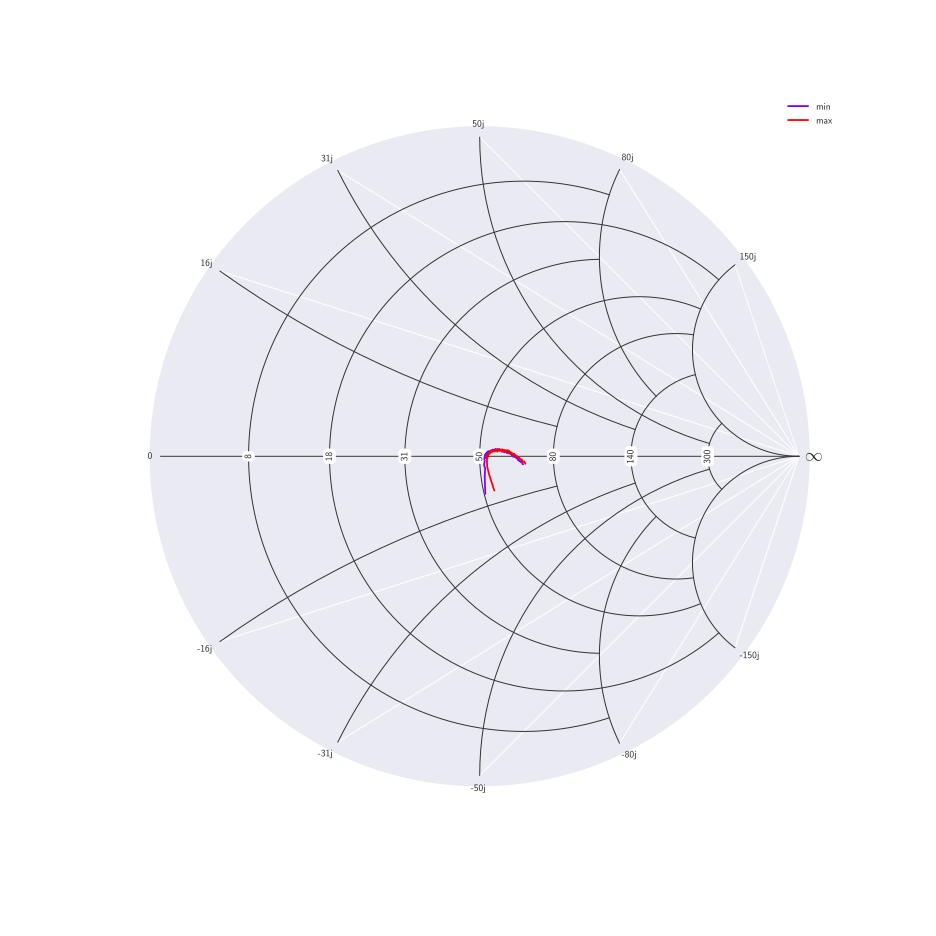
\includegraphics[width=1\textwidth]{data/images/messungen/input_Z_A8331}
    \caption{Inputimpedanz des A8331. Es sind jeweils die minimale und maximale gemessene Impedanz über alle Verstärkungen gesehen zu einer Frequenz dargestellt.}
    \label{fig:Z_in_A8331}
\end{center}
\end{figure}

Die Verstärkung sieht sehr gut aus wie Grafik \ref{fig:T_A8331} zeigt. Die Differenz zum soll ist stets kleiner als ein Dezibel. In Anbetracht des Umstandes, dass das Datasheet lediglich variable Verstärkungen auf 0.5 dB genau garantiert, ist weniger als 1 dB Abweichung extrem gut. Zudem muss berücksichtigt werden dass das Datasheet einen Verlust auf der externen Beschaltung von 0.4 dB zwischen den Pins LON und VOL sowie LOP und VOH spezifiziert.
Somit sieht die Kurve sogar noch viel besser aus.
Hier ist noch anzumerken, dass die Kurve um den Faktor $\frac{1}{a}$ und einen Faktor 2 korrigiert wurde. Der Faktor kommt daher dass das differentielle Signal nur die halbe Signalamplitude hat. 

\begin{figure}[H]
\begin{center}
    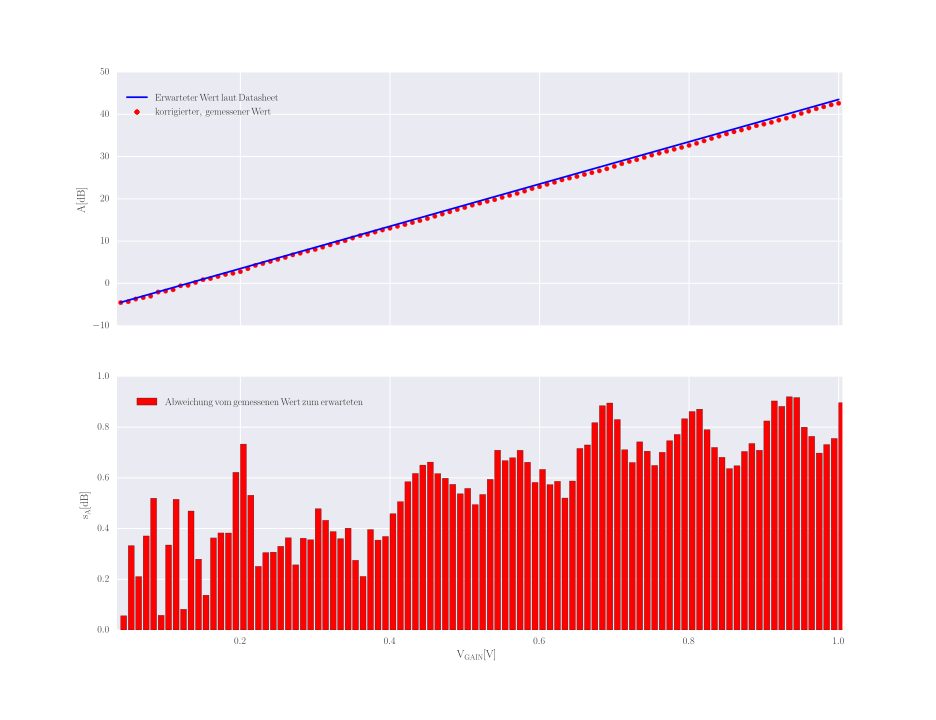
\includegraphics[width=1\textwidth]{data/images/messungen/vga_2016-12-22_30dBm_transmission2}
    \caption{Verstärkung des AD8331 gemittelt über einen 50 MHz Sweep. Ist und Soll gegenübergestellt. Zudem die Differenz zu jedem Wert.}
    \label{fig:T_A8331}
\end{center}
\end{figure}

Bei allen Messungen mit dem zweiten PCB ist der DAC nicht verbaut. Dies, da der Verdacht bestand, dass dieser viel Rauschen mit sich bringt, was nach der Erkenntniss dass der AD8331 auf dem ersten Board tatsächlich kaputt ist nicht mehr so wahrscheinlich ist. Er wurde durch eine externe Spannungsversorgung ersetzt. In weiteren Versuchen soll dieser natürlich noch genau evaluiert werden.

\subsection{ISL55210}

Da die Messungen so gut herauskamen wurde angenommen dass somit der AD8331 als Input für weitere Messungen am ISL55210 verwendet werden kann, um weiterhin auf einen Balun verzichten zu können. Mit einem twisted Pair wurden die beiden Stufen also verbunden. so kann zwar die Inputimpedanz des ISL55210 zwar nicht mehr gemessen werden, hier reichte die Transmission jedoch völlig.

Im Plot \ref{fig:T_broken_ISL55210} sieht man das Verhalten des ISL55210. Sehr unschön. Es gibt aber drei interessante Dinge zu sehen.
Erstens stimmen die gemessenen Verstärkungen über den Frequenzsweep gemittelt gut mit dem Datasheet überein wie man in Grafik \ref{fig:T_broken_mean_ISL55210} sieht.

\begin{figure}[H]
\begin{center}
    \includegraphics[width=1\textwidth]{data/images/messungen/vga_lna_2016-12-22_50dBm_20dB_transmission3}
    \caption{Verstärkung des AD8331 und ISL55210 50 MHz Sweep bei 10 verschiedenen Verstärkungen.}
    \label{fig:T_broken_ISL55210}
\end{center}
\end{figure}

\begin{figure}[H]
\begin{center}
    \includegraphics[width=1\textwidth]{data/images/messungen/vga_lna_2016-12-22_50dBm_transmission2}
    \caption{Verstärkung des AD8331 und ISL55210 gemittelt über einen 50 MHz Sweep. Ist und Soll gegenübergestellt. Zudem die Differenz zu jedem Wert.}
    \label{fig:T_broken_mean_ISL55210}
\end{center}
\end{figure}

Dies kann ein Zufall sein. Was aber viel interessanter ist, dass die Kurve zwar sehr komisch ausschaut, aber überhaupt nicht wie jene, welche beim Vorgängerprojekt gemessen wurde, wie man unschwer in Grafik \ref{fig:ganzes_system_vorganger} erkennen kann.

\begin{figure}[H]
\begin{center}
    \includegraphics[width=1\textwidth]{data/images/ganzes_system_vorganger}
    \caption{Verstärkung des AD8331 und ISL55210. Gemessen im Vorgängerprojekt.}
    \label{fig:ganzes_system_vorganger}
\end{center}
\end{figure}

Bei dieser Kurve gibt es einen Unerwarteten Abfall bei 2 MHz abwärts, was in der Vorgängerarbeit auf das aktive Impedanzmatching geschoben wurde. Dieses Verhalten konnte in den gemachten Messungen nicht nachvollzogen werden. Im Gegenteil, es wird ein starker Anstieg gemessen in diesem Bereich.

Ein dritter Punkt ist, dass der Verstärker einen unerwarteten Abfall hat je höher die Frequenz ist. Laut Datasheet sollte der Verstärker locker bis 100MHz um 28 dB verstärken. Die Kurve müsste relativ gerade ausfallen. Erst war der Gedanke da, dass es nur ein Fehle rin diesem Projekt ist. Wie sich aber zeigt bestand dieses Verhalten schon im Vorgängerprojekt, wurde jedoch nicht explizit bemerkt oder wenigstens erwähnt.

Erst viel zu spät wurde dann wenigstens noch bemerkt dass der AD8331 vollig falsch belastet wurde, da nach der Einzelmessung des AD8331 die Widerstände R7 und R8 auf 0 $\Omega$ belassen wurden statt diese korrekterweise auf 250 $\Omega$ anzupassen. Dies ist wichtg damit der AD8331 keine zu grosse last hat welche er nicht zu treiben vermag und dann komische Dinge tut.

Nach dem Wechsel sahen die Resultate waren die Resultate ganz akzeptabel!

\begin{figure}[H]
\begin{center}
    \includegraphics[width=1\textwidth]{data/images/messungen/vga_lna_2016-01-18_50dBm_10dB_HI_rez}
    \caption{Verstärkung des AD8331 und ISL55210 50 MHz Sweep bei 10 verschiedenen Verstärkungen.}
    \label{fig:T_fixed_ISL55210}
\end{center}
\end{figure}

TODO: Comment on loss of Gain at highish frequencies 

\begin{figure}[H]
\begin{center}
    \includegraphics[width=1\textwidth]{data/images/messungen/vga_lna_2016-01-18_50dBm_10dB_HI_rez_mean}
    \caption{Verstärkung des AD8331 und ISL55210 gemittelt über einen 50 MHz Sweep. Ist und Soll gegenübergestellt. Zudem die Differenz zu jedem Wert.}
    \label{fig:T_fixed_mean_ISL55210}
\end{center}
\end{figure}

Wie gut erkannt werden kann ist der Fehler der am ISL55210 entsteht grösser als derjenige, der am AD8331 entsteht. Jedoch ist der Fehler über dem ISL55210 mit weniger als 1.5 dB immernoch sehr klein. Die Abweichung zum erwarteten Wert entsteht wohl dadurch, dass zum einen die Terminierung mit 270 $\Omega$ zwischen AD8331 und ISL55210 zu hoch gewählt ist (250 $\Omega$ wären korrekt) und der Messadapter mit 250 $\Omega$, welche für den AD8331 benötigt wurden, ebenfalls einen zu hohen Widerstand hat (200 $\Omega$ wären korrekt). Wahrscheinlich der wichtigste Punkt ist aber dass die Feedbackwiderstände am AD8331 nicht eine so hohe Genauigkeit haben, dass die Effektive Verstärkung variiert.

\clearpage

\section{Resultate}
\label{sec:resultate}
Ziel des Projektes war es eigentlich, ein Redesign des bestehenden Projektes 'Software Defined Radio mit FPGA' zu machen.

Dazu war es vorab nötig ein Test-PCB zu gestalten, auf welchem korrekte Messungen gemacht werden können.
Nach einigem Einlesen in die Themata Verstärker und HF, wurde die Vorarbeit genauer untersucht.

Unter kleinlichster Berücksichtigung der Designvorgaben in den jeweiligen Datenblättern und Tipps von Analog Devices\cite{StayingWellGrounded2012}, wurde dann eine Leiterplatte gefertigt, welche die notwendigen Messanschlüsse hat und die einzelnen Baugruppen separiert. Hier wurde darauf geachtet, dass die Anordnung der Komponenten zu den Chips möglichst so angeordnet sind, wie im finalen Design notwendig, sprich nahe beim Baustein, Analoges und Digitales räumlich getrennt und mit korrektem Grounding.

Es konnten dann gute Messergebnisse zum AD8331 erzeugt werden. Probleme konnten keine festgestellt werden; die Vermutung vom Vorgängerprojekt, dass das aktive Impedanzmatching Probleme bereitet konnte nicht bestätigt werden. Der AD8331 hält alle Versprechen des Datasheets was die Verstärkung anbelangt.

Der ISL55210 konnte ebenfalls ausgemessen werden und liefert überzeugende Ergebnisse. Die Resultate sind nicht ganz so, wie laut Datasheet erwartet. Mit einer maximalen Gesamtabweichung von 2.5 dB leistet er jedoch seine Arbeit im Gesamtsystem. Hier wurden, nach anfänglich fast gleichen Ergebnissen wie bei der Vorgängerarbeit Fehler festgestellt, welche bisher nicht erkannt wurden. Nach einer korrekten Terminierung zwischen den Verstärkerstufen verhält sich der ISL55210 aber fast wie gewünscht.

Der MCP4706 war relativ einfach anzusteuern. Er verhielt sich wie erwartet und kann so eingesetzt werden.

Auch der LP38798 verhielt sich wie gewünscht und es gab keine erkennbaren Probleme mit der Spannungsversorgung. Auch hier konnten die Probleme der Vorgängerarbeit nicht reproduziert werden.

Alle genannten Fehler des Vorprojektes konnten lokalisiert und behoben oder nicht reproduziert werden.

\clearpage
\bibliography{main,example,IEEEabrv}

\end{document}

